\documentclass[12pt]{article}
\usepackage[utf8]{inputenc}
\usepackage[greek,english]{babel}
\usepackage{alphabeta}
\usepackage{fancyhdr}
\usepackage{listings}
\usepackage{mathtools}
\usepackage{xcolor}
\usepackage{float}
\usepackage{tabularx}
\usepackage[margin=0.5in]{geometry}
\usepackage[backend=bibtex]{biblatex}
\usepackage{hyperref}
\hypersetup{
	colorlinks=true,	%set true if you want colored links
	linktoc=all,		%set to all if you want both sections and subsections linked
	linkcolor=black,	%choose some color if you want links to stand out
}
\title{Εργασία Τεχνολογίας Λογισμικού -- Μέρος 2ο}
\author{Αντώνης Θωμάκος - 18390037 \\
Χρήστος Μαργιώλης - 19390133 \\
Στέφανος Στράους - 19390221}
\date{Μάιος 2022}

\begin{document}

\begin{titlepage}
        \maketitle
        \begin{figure}[t!]
        \begin{center}
        
\includegraphics[scale=1.0]{./res/uniwa-logo.pdf} \\
        \Large
        \textbf{Πανεπιστήμιο Δυτικής Αττικής} \\
        \large
        Τμήμα Μηχανικών Πληροφορικής και Ηλεκτρονικών Υπολογιστών
        \end{center}
        \end{figure}
\end{titlepage}

\renewcommand{\contentsname}{Περιεχόμενα}
\tableofcontents
\pagebreak

\section{Περιπτώσεις χρήσης}

Οι πίνακες τεκμηρίωσης πάρθηκαν από το Μέρος Α.

\subsection{Κρατήσεις εισιτηρίων}

\begin{center}
\begin{tabular}{|p{5cm}|p{12cm}|}
	\hline
	\textbf{Use Case} & Κρατήσεις εισιτηρίων (ημερομηνία, αριθμός πτήσης
	κτλ). \\
	\hline
	\textbf{Σύντομη περιγραφή} & Ο επιβάτης χρησιμοποιεί το σύστημα
	κράτησης, ορίζοντας σε αυτό στοιχεία για το εισιτήριο του όπως:
	\textit{ημερομηνία άφιξης}, \textit{ημερομηνία
	αναχώρησης}, \textit{αριθμός πτήσης},
	\textit{θέση}, \textit{αριθμός επιπλέον
	αποσκευών} κλπ. \\
	\hline
	\textbf{Actors} & Επιβάτης, Προσωπικό ταμείου (Ρεσεψιόν). \\
	\hline
	\textbf{Προαπαιτούμενα (Pre-conditions)} &
	\begin{itemize}
		\item Το σύστημα να λειτουργεί κανονικά.
		\item Το προσωπικό να κάνει την κράτηση του πελάτη.
	\end{itemize} \\
	\hline
	\textbf{Μετασυνθήκες (Post-conditions)} & Μετά την κράτηση, το
	πληροφοριακό σύστημα έχει δηλωμένα τα στοιχεία για την πτήση και ο
	πελάτης έχει εξασφαλίσει μια θέση σε αυτήν \\
	\hline
	\textbf{Κύρια ροή} &
	\begin{tabularx}{12cm}{X|X}
		\textbf{Tasks} & \textbf{Πληροφορία που απαιτείται/διαμοιράζεται} \\ 
		\hline
		Το use case ξεκινά με την εισαγωγή των στοιχείων του επιβάτη
		στο σύστημα δηλαδή των παραμέτρων του εισιτηρίου. &
		Ημερομηνία αναχώρησης, Ημερομηνία άφιξης, Αριθμός Θέσης,
		Αριθμός Πτήσης, Επιπλέον Αποσκευές, Αριθμός Εισιτηρίου. \\
		\hline
		Το σύστημα ελέγχει αν η θέση είναι διαθέσιμη. & \\
		\hline
		Το πληροφοριακό σύστημα αποκρίνεται αποθηκεύοντας τα δεδομένα
		στο σύστημα, ελέγχοντας τα ταυτόχρονα για την εγκυρότητα τους,
		όπου δίνεται ευκαιρία στον υπάλληλο να τα διορθώσει. & \\
		\hline
		Το σύστημα εκδίδει το εισιτήριο. & \\
	\end{tabularx} \\
\hline
	\textbf{Εναλλακτική ροή} &
	\begin{tabularx}{12cm}{X|X}
		\textbf{Tasks} & \textbf{Πληροφορία που απαιτείται/διαμοιράζεται} \\ 
		\hline
		Εναλλακτικά, αν η θέση δεν είναι διαθέσιμη, το σύστημα ενημερώνει τον υπάλληλο με κατάλληλο μύνημα. & \\
	\end{tabularx} \\
	\hline
\end{tabular}
\end{center}

\pagebreak
\subsection{'Ελεγχος Εγκυρότητας Εισιτηρίων (Check In)}

\begin{center}
\begin{tabular}{|p{5cm}|p{12cm}|}
	\hline
	\textbf{Use Case} & Check in εισιτηρίων πριν την πτήση. \\
	\hline
	\textbf{Σύντομη περιγραφή} & Ο υπάλληλος χρησιμοποιεί το σύστημα check
	in, ώστε να ελέγξει πριν την πτήση αν όλα τα στοιχεία του εισιτηρίου
	είναι έγκυρα και αν μπορεί να επιτρέψει στον πελάτη να επιβιβαστεί.
	Πιθανά στοιχεία είναι: \textit{Αριθμός εισιτηρίου},
	\textit{επιπλέον αποσκευές} κλπ. \\
	\hline
	\textbf{Actors} & Επιβάτης, Πράκτορας εισιτηρίων. \\
	\hline
	\textbf{Προαπαιτούμενα (Pre-conditions)} &
	\begin{itemize}
		\item Το σύστημα να λειτουργεί κανονικά.
		\item Το προσωπικό να σκανάρει το εισιτήριο του επιβάτη.
	\end{itemize} \\
	\hline
	\textbf{Μετασυνθήκες (Post-conditions)} & Μετά τον έλεγχο, το προσωπικό
	μπορεί να επιτρέψει την είσοδο του επιβάτη στο αεροπλάνο. \\
	\hline
	\textbf{Κύρια ροή} &
	\begin{tabularx}{12cm}{X|X}
		\textbf{Tasks} & \textbf{Πληροφορία που απαιτείται/διαμοιράζεται} \\ 
		\hline
		Το use case ξεκινά με το σκανάρισμα του εισιτηρίου από τον
		υπάλληλο. &
		Αριθμός Εισιτηρίου, Αριθμός Θέσης, Επιπλέον Αποσκευές. \\
		\hline
		Το πληροφοριακό σύστημα αποκρίνεται ελέγχοντας αν ταυτίζονται
		τα δεδομένα του εισιτηρίου με αυτά στο σύστημα. & \\
		\hline
		Ο υπάλληλος αποφασίζει αν μπορεί να επιβιβαστεί ο πελάτης. & \\
	\end{tabularx} \\
	\hline
	\textbf{Εναλλακτική ροή} &
	\begin{tabularx}{12cm}{X|X}
		\textbf{Tasks} & \textbf{Πληροφορία που απαιτείται/διαμοιράζεται} \\ 
		\hline
		Εναλλακτικά, σε περίπτωση άκυρου εισητιρίου ο επιβάτης δεν
		μπορεί να εισέλθει στην πτήση. & \\
	\end{tabularx} \\
	\hline
\end{tabular}
\end{center}

\pagebreak
\subsection{Πληροφορίες Πτήσης (F.I.D.S.)}

\begin{center}
\begin{tabular}{|p{5cm}|p{12cm}|}
	\hline
	\textbf{Use Case} & Εμφάνιση πληροφοριών για τις πτήσεις στις οθόνες
	του αεροδρομίου (Αριθμός πτήσης, κατάσταση πτήσης, πύλη κτλ). \\
	\hline
	\textbf{Σύντομη περιγραφή} & Το σύστημα F.I.D.S. λαμβάνει πληροφορίες
	από διεθνής φορείς, και έπειτα ανανεώνει την τοπική βάση δεδομένων, η
	οποία μοιράζεται σε κάθε οθόνη του αεροδρομίου ώστε να υπάρχει έγκυρη
	ενημέρωση των επιβατών με στοιχεία όπως: \textit{ώρα
	άφιξης/αναχώρησης}, \textit{αριθμός πτήσης},
	\textit{κατάσταση πτήσης}, \textit{πύλη},
	\textit{προορισμός} κλπ. \\
	\hline
	\textbf{Actors} & Οθόνη, Πληροφοριακό σύστημα. \\
	\hline
	\textbf{Προαπαιτούμενα (Pre-conditions)} &
	\begin{itemize}
		\item Το σύστημα να λειτουργεί κανονικά.
		\item Να υπάρχουν έγκυρες πληροφορίες για τις πτήσεις από
			κάποιο διεθνή σύστημα πληροφοριών.
	\end{itemize} \\
	\hline
	\textbf{Μετασυνθήκες (Post-conditions)} & Το σύστημα μετά το use case,
	έχει εμφανίσει όλες τις πληροφορίες σχετικές με την πτήση στις οθόνες
	του F.I.D.S. \\
	\hline
	\textbf{Κύρια ροή} &
	\begin{tabularx}{12cm}{X|X}
		\textbf{Tasks} & \textbf{Πληροφορία που απαιτείται/διαμοιράζεται} \\ 
		\hline
		Το use case ξεκινά όταν το πληροφοριακό σύστημα κατεβάζει
		δεδομένα από την διεθνή βάση δεδομένων πτήσεων, και τα φορτώνει
		στην τοπική βάση δεδομένων. &
		'Ωρα άφιξης/αναχώρησης, αριθμός πτήσης, κατάσταση πτήσης, πύλη,
		προορισμός \\
		\hline
		Τα δεδομένα πτήσεων έπειτα στέλνονται από την βάση δεδομένων
		ξεχωριστά σε κάθε οθόνη στο αεροδρόμιο & \\
	\end{tabularx} \\
	\hline
	\textbf{Εναλλακτική ροή} &
	\begin{tabularx}{12cm}{X|X}
		\textbf{Tasks} & \textbf{Πληροφορία που απαιτείται/διαμοιράζεται} \\ 
		\hline
		Δεν υπάρχει εναλλακτικό σενάριο πέραν του 1 και 2, αν δεν
		γίνουν αυτά το σύστημα δεν λειτουργεί. & \\
	\end{tabularx} \\
	\hline
\end{tabular}
\end{center}

\pagebreak
\section{UML Activity διαγράμματα}

Τα παρακάτω διαγράμματα αντιστοιχούν στις τρεις παραπάνω περιπτώσεις χρήσεις,

\subsection{Κρατήσεις εισιτηρίων}
\begin{figure}[H]
	\centering
	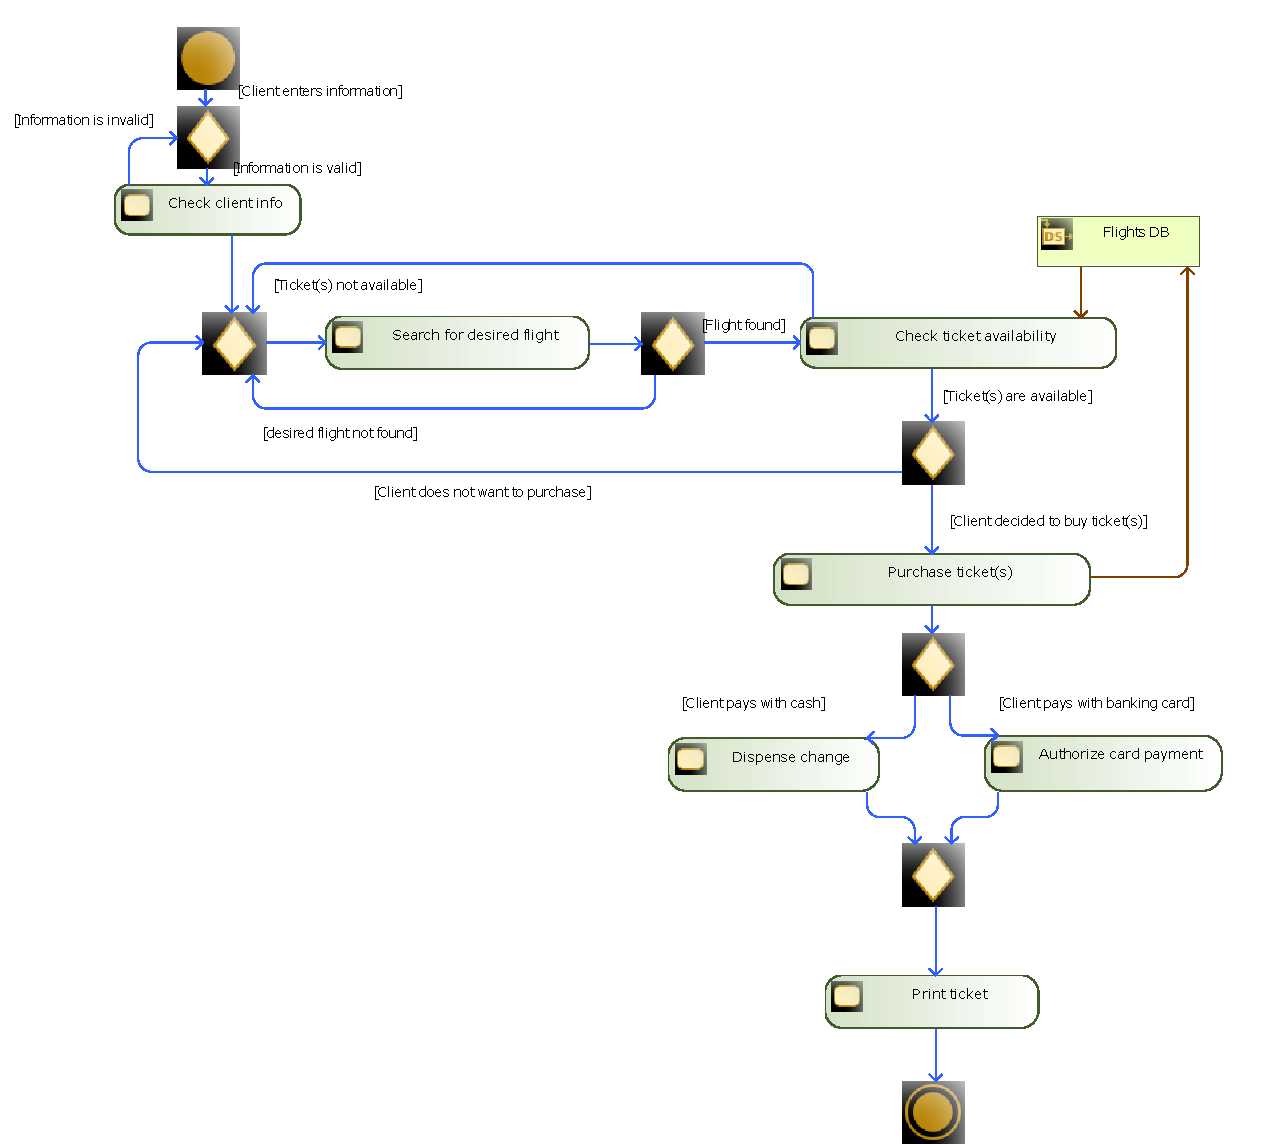
\includegraphics[width=\linewidth]{./res/adiag1.pdf}
	\caption{Activity diagram 1 -- Κρατήσεις εισιτηρίων.}
\end{figure}

\subsection{'Ελεγχος Εγκυρότητας Εισιτηρίων (Check In)}
\begin{figure}[H]
	\centering
	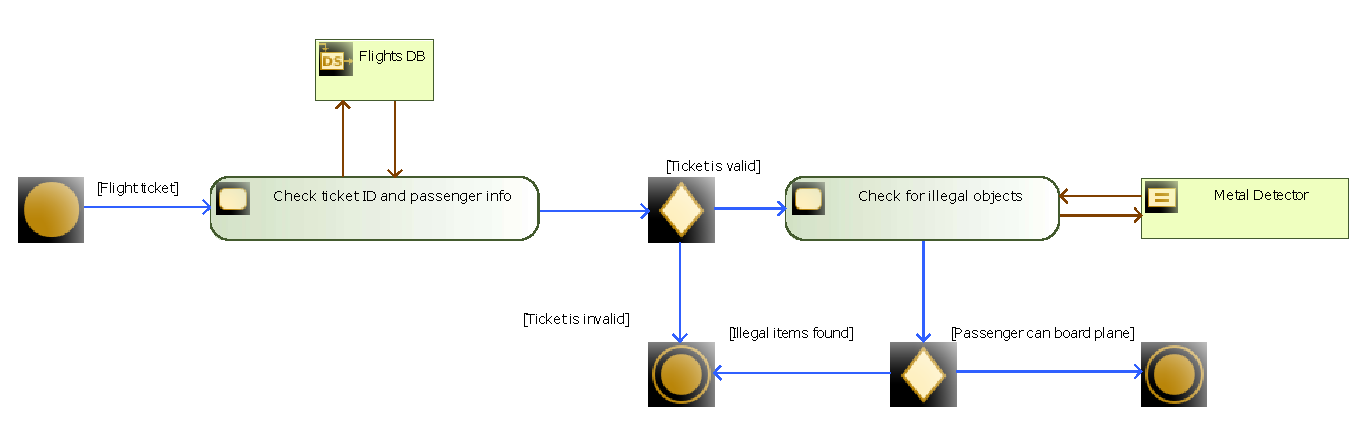
\includegraphics[width=\linewidth]{./res/adiag2.pdf}
	\caption{Activity diagram 2 -- Check in.}
\end{figure}

\subsection{Πληροφορίες Πτήσης (F.I.D.S.)}
\begin{figure}[H]
	\centering
	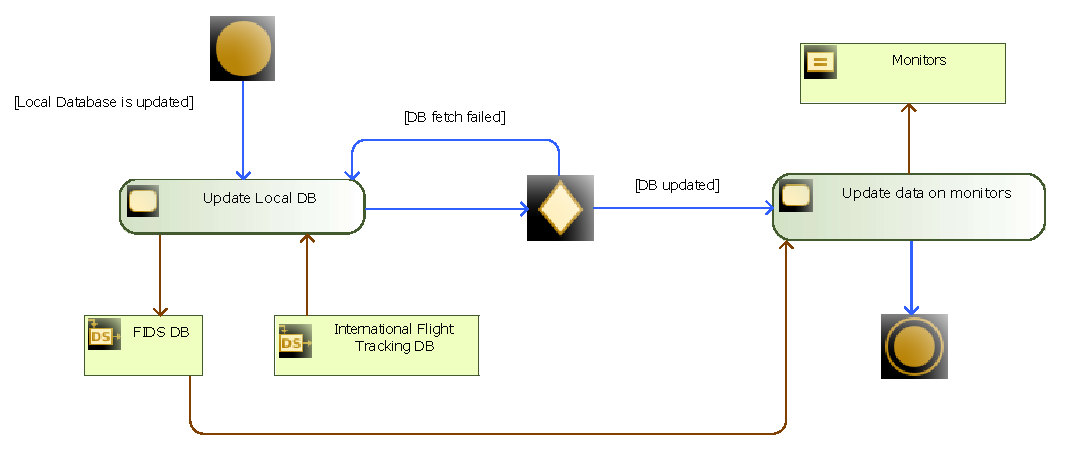
\includegraphics[width=\linewidth]{./res/adiag3.pdf}
	\caption{Activity diagram 3 -- F.I.D.S.}
\end{figure}

\end{document}
